\documentclass[11pt,a4paper]{article}

\usepackage[a4paper,left=2.2cm,right=2.2cm,top=2.4cm,bottom=2.4cm]{geometry}
\usepackage[T1]{fontenc}
\usepackage[utf8]{inputenc}
\usepackage{lmodern}
\usepackage{microtype}
\usepackage{booktabs}
\usepackage{tabularx}
\usepackage{array}
\usepackage{enumitem}
\usepackage{hyperref}
\usepackage{xcolor}
\usepackage{titlesec}
\usepackage{fancyhdr}
\usepackage{lastpage}
\usepackage{tcolorbox}
\usepackage{amsmath}
\usepackage{amssymb}
\usepackage{tikz}
\usetikzlibrary{positioning}
\tcbuselibrary{skins,breakable}

\hypersetup{
  colorlinks=true,
  linkcolor=black,
  urlcolor=black,
  pdftitle={PHOENIX evaluatiestudie - HCP-PRE-05 (C05)},
  pdfauthor={Stijn Van Severen -- Universiteit Gent}
}

\definecolor{PrimaryBlue}{HTML}{1D4ED8}
\definecolor{DarkBlue}{HTML}{1E3A5F}
\definecolor{SlateMid}{HTML}{475569}
\definecolor{ForestGreen}{HTML}{047857}
\definecolor{RichPurple}{HTML}{6D28D9}
\definecolor{GoldAmber}{HTML}{B45309}
\definecolor{StrongRed}{HTML}{B91C1C}
\definecolor{SoftBG}{HTML}{F8FAFC}
\definecolor{BorderGrey}{HTML}{CBD5E1}
\definecolor{AccentBlue}{HTML}{DBEAFE}
\definecolor{AccentGreen}{HTML}{D1FAE5}
\definecolor{AccentAmber}{HTML}{FEF3C7}
\definecolor{AccentPurple}{HTML}{EDE9FE}
\definecolor{AccentTeal}{HTML}{CCFBF1}
\definecolor{AccentOrange}{HTML}{FFEDD5}

\titleformat{\section}{\Large\bfseries\color{DarkBlue}}{\thesection}{0.7em}{}[\vspace{-0.2em}\color{PrimaryBlue}\rule{\textwidth}{0.6pt}]
\titleformat{\subsection}{\large\bfseries\color{PrimaryBlue}}{\thesubsection}{0.6em}{}
\titleformat{\subsubsection}{\normalsize\bfseries\color{ForestGreen}}{\thesubsubsection}{0.5em}{}

\setlist[itemize]{topsep=3pt,itemsep=2pt,leftmargin=1.4em}
\setlist[enumerate]{topsep=3pt,itemsep=2pt,leftmargin=1.6em}
\setlength{\parskip}{0.45em}
\setlength{\parindent}{0pt}
\renewcommand{\arraystretch}{1.28}

\pagestyle{fancy}
\fancyhf{}
\fancyhead[L]{\small\color{SlateMid}PHOENIX evaluatiestudie -- Fase 1}
\fancyhead[R]{\small\color{SlateMid}\textbf{HCP-PRE-05}\quad C05}
\fancyfoot[C]{\small Pagina \thepage\ van \pageref{LastPage}}
\renewcommand{\headrulewidth}{0.3pt}
\renewcommand{\footrulewidth}{0pt}

\newtcolorbox{complaintbox}[1][]{
  colback=blue!3,colframe=PrimaryBlue,
  boxrule=0.8pt,arc=2.5mm,breakable,
  left=10pt,right=10pt,top=8pt,bottom=8pt,
  fonttitle=\small\bfseries\color{PrimaryBlue},
  title=Casusvignet,#1
}
\newtcolorbox{contextbox}[1][]{
  colback=green!3,colframe=ForestGreen,
  boxrule=0.6pt,arc=2mm,breakable,
  left=8pt,right=8pt,top=7pt,bottom=7pt,
  fonttitle=\small\bfseries\color{ForestGreen},
  title=Gestandaardiseerde context,#1
}
\newtcolorbox{instrbox}[1][]{
  colback=SoftBG,colframe=BorderGrey,
  boxrule=0.5pt,arc=1.5mm,breakable,
  left=8pt,right=8pt,top=7pt,bottom=7pt,
  fonttitle=\bfseries\color{SlateMid},#1
}
\newtcolorbox{monitorbox}{
  colback=SoftBG,colframe=BorderGrey,
  boxrule=0.5pt,arc=1.5mm,breakable,
  left=6pt,right=6pt,top=5pt,bottom=5pt
}
\newtcolorbox{responsebox}{
  colback=yellow!5,colframe=GoldAmber,
  boxrule=0.7pt,arc=2mm,breakable,
  left=10pt,right=10pt,top=9pt,bottom=9pt,
  fonttitle=\small\bfseries\color{RichPurple},
  title=Uw antwoord
}
\newtcolorbox{voorbeeldbox}[3][]{
  colback=AccentPurple,colframe=RichPurple,
  boxrule=0.8pt,arc=2.5mm,breakable,
  left=10pt,right=10pt,top=9pt,bottom=9pt,
  fonttitle=\small\bfseries\color{RichPurple},
  halign title=center,
  title={Uitgewerkt voorbeeld -- #2 -- Nadia (38-jarige verpleegkundige)\\[1pt]%
    {\footnotesize\itshape\color{white}#3}},#1
}

\tikzset{
  crnode/.style={
    draw=PrimaryBlue,fill=AccentBlue,rounded corners=2pt,
    text width=3.55cm,minimum height=0.76cm,
    font=\fontsize{6.5}{8}\selectfont\bfseries\color{DarkBlue},
    align=center,inner sep=3pt
  },
  prnode/.style={
    draw=ForestGreen,fill=AccentTeal,rounded corners=2pt,
    text width=3.55cm,minimum height=0.76cm,
    font=\fontsize{6.5}{8}\selectfont\bfseries\color{ForestGreen},
    align=center,inner sep=3pt
  },
  smcrnode/.style={
    draw=PrimaryBlue,fill=AccentBlue,rounded corners=2pt,
    text width=2.9cm,minimum height=0.70cm,
    font=\fontsize{6.0}{7.5}\selectfont\bfseries\color{DarkBlue},
    align=center,inner sep=2pt
  },
  smprnode/.style={
    draw=ForestGreen,fill=AccentTeal,rounded corners=2pt,
    text width=2.9cm,minimum height=0.70cm,
    font=\fontsize{6.0}{7.5}\selectfont\bfseries\color{ForestGreen},
    align=center,inner sep=2pt
  },
}

\newcommand{\writeline}{\vspace{0.22em}\noindent\rule{\linewidth}{0.25pt}\vspace{0.42em}\par}

\newcommand{\symptoomslot}[1]{%
\vspace{0.25em}\noindent
\begin{tcolorbox}[colback=SoftBG,colframe=BorderGrey,boxrule=0.4pt,arc=1.5mm,left=8pt,right=8pt,top=5pt,bottom=5pt]%
\small\textbf{\color{SlateMid}Symptoom #1}\hspace{1em}%
\textbf{Label:}\hspace{0.5em}\rule{0.56\linewidth}{0.25pt}%
\end{tcolorbox}%
}

\newcommand{\behandelingsoptieslot}[1]{%
\vspace{0.25em}\noindent
\begin{tcolorbox}[colback=SoftBG,colframe=BorderGrey,boxrule=0.4pt,arc=1.5mm,left=8pt,right=8pt,top=5pt,bottom=5pt]%
\small\textbf{\color{SlateMid}Behandelingsoptie #1}\hspace{1em}%
\textbf{Label:}\hspace{0.5em}\rule{0.56\linewidth}{0.25pt}%
\end{tcolorbox}%
}

\newcommand{\rankbox}[1]{%
\vspace{0.22em}\noindent
\begin{tikzpicture}[baseline=3pt]
  \node[draw=DarkBlue,fill=AccentBlue,rounded corners=3pt,minimum width=2.5cm,minimum height=0.72cm,font=\small\bfseries\color{DarkBlue},align=center] {Prioriteit #1};
\end{tikzpicture}
\hspace{0.7em}\rule{0.60\linewidth}{0.25pt}\par\vspace{0.05em}
}

\newcommand{\checkitemBFS}[2]{%
\noindent\small\textbf{#1.}\hspace{0.45em}$\square$\hspace{0.4em}#2\par\vspace{0.20em}}

\newcommand{\messagelines}{\writeline\writeline\writeline\writeline}

\begin{document}

% ── TITELPAGINA ─────────────────────────────────────────────────────────────
\thispagestyle{fancy}
\vspace*{0.3cm}

\begin{tcolorbox}[
  colback=DarkBlue,colframe=DarkBlue,
  arc=3mm,left=14pt,right=14pt,top=12pt,bottom=12pt,
  width=\textwidth
]
\centering
{\fontsize{22}{28}\selectfont\bfseries\color{white}
PHOENIX evaluatiestudie\\[0.3em]
\fontsize{15}{20}\selectfont\color{AccentBlue}
Fase 1 -- onafhankelijke expertgeneratie\\[0.2em]
\fontsize{12}{16}\selectfont\color{white}
\textit{Instrument voor Zorgprofessionals}
}
\end{tcolorbox}

\vspace{0.6cm}

\begin{center}
\begin{tcolorbox}[
  colback=AccentBlue,colframe=PrimaryBlue,
  arc=2.5mm,boxrule=1.2pt,left=12pt,right=12pt,top=10pt,bottom=10pt,
  width=0.86\textwidth
]
\centering
{\large\bfseries\color{DarkBlue}Deelnemerscode: \texttt{HCP-PRE-05}}\\[0.5em]
{\normalsize\color{SlateMid}
Toegewezen casus:\quad
\textbf{\color{PrimaryBlue}C05} (25-jarige postgraduaatsstudent)
}
\end{tcolorbox}
\end{center}

\vspace{0.5cm}

\begin{center}
\begin{tcolorbox}[
  colback=SoftBG,colframe=BorderGrey,
  arc=2mm,left=10pt,right=10pt,top=9pt,bottom=9pt,
  width=0.92\textwidth
]
\small\renewcommand{\arraystretch}{1.28}
\begin{tabularx}{\textwidth}{@{}>{\bfseries\raggedright\arraybackslash}p{0.29\textwidth}X@{}}
Studie & Evaluatie van de klinische kwaliteit van een ontologiegebaseerd multi-agentsysteem voor gepersonaliseerde digitale geestelijke gezondheidszorg \\
Instelling & Universiteit Gent -- Faculteit Psychologie en Pedagogische Wetenschappen \\
Onderzoeker & Stijn Van Severen (masterproefstudent) \\
Promotoren & Prof.\ Dr.\ Geert Crombez; Dr.\ Annick De Paepe \\
Contact & \texttt{stijn.vanseveren@ugent.be} \\
Geschatte duur & Ongeveer 20--25 minuten voor de casus (inclusief leestijd instructies) \\
\end{tabularx}
\end{tcolorbox}
\end{center}

\vspace{0.4cm}

\begin{center}
\begin{tcolorbox}[
  colback=SoftBG,colframe=BorderGrey,
  arc=2mm,left=10pt,right=10pt,top=9pt,bottom=9pt,
  width=0.92\textwidth
]
\textbf{\color{PrimaryBlue}Doel van deze bundel}

\medskip\small
U neemt deel aan een evaluatiestudie waarin zorgprofessionals onafhankelijk dezelfde
vijf klinische redeneerstappen uitvoeren als een geautomatiseerd multi-agentsysteem. Uw antwoorden
vormen het menselijke referentiecorpus voor een latere dubbelblinde vergelijking
met systeemoutput.

\smallskip
Voor uw casus vult u dezelfde vijf delen in: (1) operationalisering,
(2) initieel observatiemodel, (3) prioritering van behandeldoelen, (4) verfijning van
EMA-metingen en (5) een mobiele coachingsboodschap.

\smallskip
\textbf{We vragen uw eigen klinische oordeelsvorming.} Antwoord zoals u dat in een
reele professionele context zou doen, maar werk strikt volgens de instructies op de
volgende pagina.
\end{tcolorbox}
\end{center}

\vspace{0.4cm}

\begin{center}
\begin{tcolorbox}[
  colback=AccentAmber,colframe=GoldAmber,
  arc=2mm,boxrule=0.7pt,left=10pt,right=10pt,top=8pt,bottom=8pt,
  width=0.90\textwidth
]
\small\centering
\textbf{\color{GoldAmber}Vertrouwelijkheid:} uw antwoorden worden voor analyse
geanonimiseerd en uitsluitend gebruikt binnen deze masterproefstudie. Deelname is
vrijwillig; u kan zich op elk moment terugtrekken door contact op te nemen met de
onderzoeker.
\end{tcolorbox}
\end{center}

\vfill
\newpage
\tableofcontents
\newpage


% ── INSTRUCTIEPAGINA ─────────────────────────────────────────────────────────
\section{Instructiepagina}

\subsection*{Het PHOENIX-systeem en de context van deze studie}

\textbf{PHOENIX} (Personalized Hierarchical Optimization Engine for Navigating
Insightful eXplorations) is een multi-agentsysteem ontwikkeld als onderdeel van
een masterproef in de psychologie aan de Universiteit Gent. Het systeem verwerkt
een vrije klachttekst en doorloopt vijf opeenvolgende klinische redeneerstappen
die de kern vormen van een gepersonaliseerde, longitudinale digitale interventie.

Het theoretische kader van PHOENIX steunt op het \textbf{netwerk-analytisch model
van psychopathologie}: psychische klachten worden niet
als uitingen van een latente stoornis beschouwd, maar als een \emph{dynamisch
netwerk van onderling samenhangende klachtcomponenten}. Een sleutelbegrip daarbinnen
is het onderscheid tussen \textbf{symptomen} (klacht- en toestandsdimensies die
beschrijven wat er mis gaat bij de persoon) en \textbf{behandelingsopties}
(modificeerbare gedragsvariabelen die de symptomen causaal beinvloeden en als
behandeldoel kunnen dienen).

\vspace{0.4em}
\begin{instrbox}[title={Kerndefinities: symptoom versus behandelingsoptie}]
\small
\textbf{Symptoom (S):} een klinisch relevante, momentaan aanwezige
\emph{klacht- of toestandsdimensie} van de persoon die herhaald meetbaar is via
dagelijkse EMA. Symptomen zijn de \emph{uitkomstvariabelen} in het netwerk -- ze
beschrijven \emph{wat er mis gaat} (bijv.\ intrusieve obsessies, paniekepisoden,
prestatieangst). Symptomen zijn geen gedragingen of interventies.

\medskip
\textbf{Behandelingsoptie (BO):} een \emph{modificeerbare gedrags- of procesvariabele}
die plausibel causaal ingrijpt op een of meerdere symptomen en dagelijks meetbaar
is via een korte EMA-vraag. Behandelingsopties zijn de \emph{ingreepvariabelen} in het
netwerk -- ze beschrijven \emph{wat veranderbaar is} (bijv.\ compulsie-uitstel,
geplande exposure, post-event verwerking). Een behandelingsoptie is \emph{nooit een symptoom zelf},
maar een gedrag, strategie of omgevingsfactor die het symptoom beinvloedt.

\medskip\small
\textit{Voorbeelden ter verduidelijking:}
\begin{itemize}[topsep=1pt,itemsep=0pt]
\item \textbf{Symptoom:} intrusieve obsessies, prestatieangst, post-event ruminatie, vermijding van zichtbaarheid.
\item \textbf{Behandelingsoptie:} compulsie-uitstel (min), geplande exposurestap (ja/nee),
post-event verwerkingsoefening (ja/nee), vermijdingslogging (aantal).
\end{itemize}
\end{instrbox}

\vspace{0.4em}
\begin{instrbox}[title={Ecological Momentary Assessment (EMA) -- basisprincipes}]
\small
\textbf{EMA} is een methode waarbij personen vaak meerdere keren per dag hun actuele
toestand of gedrag rapporteren via een mobiele applicatie. In PHOENIX wordt EMA
gebruikt om zowel symptomen als behandelingsopties dagelijks te monitoren over een periode
van meerdere weken.

Een goede EMA-variabele voldoet aan vier vereisten:
\begin{itemize}[topsep=2pt,itemsep=1pt]
\item \textbf{Dagelijks rapporteerbaar:} via een korte vraag op de smartphone, bijv.\ (ja/nee, aantal, minuten of 0--10).
\item \textbf{Dynamisch en veranderbaar:} geen vaste trek, diagnose of stabiel achtergrondkenmerk.
\item \textbf{Klinisch relevant:} toont binnen-persoonsvariatie die therapeutisch informatief is.
\item \textbf{Onderscheid symptoom vs.\ behandelingsoptie:} klachtdimensies zijn symptomen; modificeerbare gedragingen zijn behandelingsopties.
\end{itemize}
\end{instrbox}

\vspace{0.4em}
\begin{instrbox}[title={Het bipartiet netwerk: structuur van het observatiemodel}]
\small
Na 21 dagen EMA-monitoring construeert PHOENIX een \textbf{bipartiet netwerk}:
een graaf met twee kolommensets en gewogen verbindingen daartussen.
\begin{itemize}[topsep=2pt,itemsep=1pt]
\item \textbf{Linkse kolom -- Behandelingsopties (BO):} de modificeerbare variabelen.
\item \textbf{Rechtse kolom -- Symptomen (S):} de klacht- en toestandsdimensies.
\item \textbf{Kanten:} de richting loopt van behandelingsoptie naar symptoom (BO $\rightarrow$ S).
Een \emph{blauwe} rand duidt op een positief verband (behandelingsoptie vergroot het symptoom),
een \emph{rode} rand op een negatief verband (behandelingsoptie verkleint het symptoom).
Lijndikte is proportioneel aan de sterkte van het empirische verband uit de monitoringdata.
\end{itemize}
In \textbf{Deel 3} rangschikt u de behandelingsopties op behandelprioriteit op basis van
dit netwerk en de monitoringsamenvatting.
\end{instrbox}

\vspace{0.5em}

\subsection*{Overzicht van de vijf taken}

\begin{center}
\renewcommand{\arraystretch}{1.36}
\small
\begin{tabular}{@{}>{\bfseries\color{PrimaryBlue}}p{0.05\textwidth}>{\bfseries}p{0.30\textwidth}p{0.38\textwidth}p{0.13\textwidth}@{}}
\toprule
Stap & Klinische taak & Wat u doet & Richttijd \\
\midrule
-- & Instructies lezen & Lees de instructiepagina aandachtig door & $\approx$\,5 min \\
1 & Operationalisering & Identificeer 2--6 \textbf{symptoomlabels} (klachtdimensies) & $\approx$\,3 min \\
2 & Initieel observatiemodel & Genereer 3--5 \textbf{behandelingsoptielabels} (modificeerbaar, EMA-geschikt) & $\approx$\,3 min \\
3 & Behandeldoelprioritering & Rangschik alle 5 \textbf{behandelingsopties} van hoog naar laag behandelprioriteit & $\approx$\,4 min \\
4 & Verfijnd observatiemodel & Selecteer exact 6 \textbf{EMA-items} (2 per behandeldoel) uit de lijst van 20 & $\approx$\,4 min \\
5 & Mobiele coaching & Schrijf een korte patientgerichte boodschap voor de app & $\approx$\,4 min \\
\midrule
 & \textbf{Totaal (1 casus)} & & \textbf{20--25 min} \\
\bottomrule
\end{tabular}
\end{center}

\vspace{0.5em}
\begin{instrbox}[title={Werkwijze -- strikt te volgen}]
\begin{enumerate}[topsep=1pt,itemsep=2pt]
\item \textbf{Werk sequentieel: Deel 1 $\rightarrow$ Deel 5.}
Ga pas naar een volgend deel wanneer het huidige deel volledig is afgewerkt.
\item \textbf{Gebruik geen generatieve AI, schrijfhulpmiddelen, richtlijnen of collegaoverleg.}
Extern gebruik ondermijnt de methodologische validiteit en de blind scoringswaarde van de studie.
\item \textbf{Gebruik in latere delen uitsluitend de meegeleverde gestandaardiseerde context.}
Die is bewust vastgezet zodat alle deelnemers op identieke input reageren en vergelijkbaar zijn.
\item \textbf{Herwerk eerdere antwoorden niet retroactief} nadat u latere context hebt gezien.
\item \textbf{Noteer of typ rechtstreeks in de voorziene antwoordzones.}
Onleesbare of ambigu geformuleerde antwoorden bemoeilijken latere blinde beoordeling.
\item \textbf{Werk ook bij beperkte informatie.} Klinische teksten bevatten vaak onvoldoende informatie voor definitieve conclusies. Geef \emph{altijd} een antwoord op basis van de beschikbare informatie en uw klinisch oordeel. Laat geen velden blanco zonder reden.
\end{enumerate}
\end{instrbox}

\newpage


% ══════════════════════════════════════════════════════════════════════════════
\section{Deel 1: Operationalisering van de mentale gezondheidstoestand}

\begin{tcolorbox}[colback=blue!3,colframe=PrimaryBlue,arc=2.5mm,boxrule=0.9pt,
  left=10pt,right=10pt,top=9pt,bottom=9pt]
\textbf{\color{PrimaryBlue}Instructies Deel 1}

\smallskip\small
\textbf{Opdracht:} identificeer de belangrijkste actuele klacht- en toestandsdimensies
(\textbf{symptomen}) in de klachttekst en noteer voor elke dimensie uitsluitend een
\textbf{kort symptoomlabel}.

\textbf{Wat is een symptoom?}
Een symptoom is een \emph{klacht- of toestandsdimensie} die beschrijft \emph{wat er
mis gaat} bij de persoon. Het is \emph{geen} behandeling, geen gedrag en geen oorzaak,
maar een actuele toestandsbeschrijving:
\begin{itemize}[topsep=2pt,itemsep=1pt]
\item momenteel aanwezig bij de persoon (niet hypothetisch of anamnestisch),
\item onderscheidbaar van andere klachtdimensies (niet overlappend),
\item in principe herhaald meetbaar via dagelijkse zelfrapportage (EMA),
\item op DSM-5-TR/ICD-11-niveau: concreet genoeg om afzonderlijk te meten (bijv.\ ``inslaapmoeilijkheden'', niet het brede ``slaapstoornis''), maar niet te atomair (niet ``wakker om 3u00'' als apart symptoom).
\end{itemize}

\textbf{Voorbeelden van goede symptoomlabels:}
intrusieve obsessies, compulsief controlegedrag, prestatieangst, post-event ruminatie,
vermijding van zichtbaarheid, anticipatieangst, tijdsbelasting door rituelen.

\textbf{Let op:} gedragingen (bijv.\ ``compulsie-uitstel''), oorzaken (bijv.\ ``perfectionisme'')
en behandelstrategieën zijn \emph{geen} symptomen maar behandelingsopties -- die horen in Deel 2.

\textbf{Antwoordformat:} label van 2--5 woorden, zonder beschrijvende zin.
Noteer per casus \textbf{2--6 symptomen}. Laat ongebruikte velden leeg.

\medskip
\textit{\textbf{Zie het uitgewerkte voorbeeld hieronder} voor een concrete illustratie van wat een correct symptoomlabel is.}
\end{tcolorbox}

\vspace{0.5em}
\nopagebreak[4]

% ── VOORBEELD DEEL 1 ─────────────────────────────────────────────────────────
\begin{voorbeeldbox}{Deel 1: Operationalisering}{Hoe formuleert u een correct symptoomlabel?}
\small
\textbf{Klacht (verkorte versie):} \textit{``De afgelopen vijf maanden slaap ik slecht:
ik lig lang wakker en word vroeg wakker. Overdag ben ik moe en prikkelbaar. Ik beweeg
bijna niet meer en zie vrienden nauwelijks nog.''}

\medskip
\textbf{Correct ingevulde symptoomlabels} (elk één klachtdimensie, expliciet uit de tekst):
\begin{itemize}[topsep=2pt,itemsep=1pt]
\item \textbf{S-1}\enspace Inslaapmoeilijkheden
  \hfill\textit{(``lig lang wakker'' $\rightarrow$ afzonderlijk meetbaar)}
\item \textbf{S-2}\enspace Vroegochtendontwaak
  \hfill\textit{(``word vroeg wakker'' $\rightarrow$ DSM-5-TR: early morning awakening; onderscheidbaar van S-1)}
\item \textbf{S-3}\enspace Vermoeidheid overdag
  \hfill\textit{(``moe overdag'' $\rightarrow$ toestandsdimensie)}
\item \textbf{S-4}\enspace Prikkelbaarheid
  \hfill\textit{(``prikkelbaar'' $\rightarrow$ emotioneel symptoom, los van S-3)}
\item \textbf{S-5}\enspace Sociale terugtrekking
  \hfill\textit{(``zie vrienden nauwelijks'' $\rightarrow$ klachtpatroon)}
\end{itemize}

\medskip
\textbf{\color{StrongRed}Dit zijn GEEN symptoomlabels} (horen in Deel 2 als behandelingsoptie):
\begin{itemize}[topsep=1pt,itemsep=0pt]
\item \textit{``Weinig bewegen''} $\rightarrow$ modificeerbaar gedrag, geen klacht; hoort bij Deel 2.
\item \textit{``Slaapproblemen''} $\rightarrow$ te breed: splits naar meetbare dimensies (zie S-1 en S-2).
\end{itemize}
\end{voorbeeldbox}

\vspace{0.5em}

\newpage

\subsection*{Casus 1: 25-jarige postgraduaatsstudent}

\begin{complaintbox}[title={Casus 1: 25-jarige postgraduaatsstudent; duur: 18 maanden}]
\small ``De afgelopen anderhalf jaar word ik dagelijks gekweld door opdringerige gedachten over het per ongeluk schaden van anderen -- dat ik iemand aangereden heb, een gasfornuis open heb laten staan, of een deur niet afgesloten heb. Zodra zo'n gedachte opkomt, kan ik niet ophouden met mentaal controleren: ik ga de situatie telkens opnieuw na in mijn hoofd en stel mezelf steeds dezelfde vragen totdat ik tijdelijk gerustgesteld ben. Dit ritueel kost mij dagelijks twee tot vier uur. Inmiddels vermijd ik steeds meer situaties die deze gedachten uitlokken -- zoals autorijden of het als laatste verlaten van een ruimte -- en vraag ik regelmatig aan anderen of er niets mis is gegaan. Die geruststelling helpt even, maar de gedachten komen sterker terug.''
\end{complaintbox}

\begin{responsebox}
\small\textbf{Opdracht:} noteer \textbf{2--6 symptoomlabels} voor deze casus.
Gebruik enkel korte labels (2--5 woorden); voeg geen beschrijving toe.

\symptoomslot{1}
\symptoomslot{2}
\symptoomslot{3}
\symptoomslot{4}
\symptoomslot{5}
\symptoomslot{6}
\end{responsebox}

\vspace{0.6em}

\newpage


% ══════════════════════════════════════════════════════════════════════════════
\section{Deel 2: Initieel observatiemodel (bipartiet netwerk)}

\begin{tcolorbox}[colback=green!3,colframe=ForestGreen,arc=2.5mm,boxrule=0.9pt,
  left=10pt,right=10pt,top=9pt,bottom=9pt]
\textbf{\color{ForestGreen}Instructies Deel 2}

\smallskip\small
\textbf{Opdracht:} genereer \textbf{3--5 behandelingsoptielabels} die samen het
\textbf{initieel observatiemodel} voor deze casus vormen.

\textbf{Wat is een behandelingsoptie in deze context?}
Een behandelingsoptie is een \emph{modificeerbare gedrags- of procesvariabele} die beschrijft
\emph{wat de persoon kan veranderen}:
\begin{itemize}[topsep=2pt,itemsep=1pt]
\item \textbf{Modificeerbaar:} de persoon (of therapeut) kan er rechtstreeks op ingrijpen.
\item \textbf{EMA-geschikt:} dagelijks meetbaar via een eenvoudige vraag op de smartphone
(ja/nee, aantal, minuten of 0--10 schaal).
\item \textbf{Causaal plausibel:} klinisch aannemelijk dat de behandelingsoptie de symptomen beinvloedt.
\item \textbf{Geen symptoom:} klachtniveaus of diagnostische trekken zijn
\emph{geen} behandelingsopties.
\end{itemize}

\textbf{Voorbeelden van goede behandelingsoptielabels:}
compulsie-uitstel, geplande exposure, geruststellingszoekend gedrag, post-event verwerking,
vermijdingslogging, cognitieve naverwerking, exposureduur.

\textbf{Let op:} variabelen als ``prestatieangst'', ``ruminatie'' of ``intrusieve obsessies'' zijn
klachtdimensies (symptomen) -- geen behandelingsopties. Kies variabelen die de persoon
actief kan uitvoeren of aanpassen.

\textbf{Antwoordformat:} enkel een label van 2--6 woorden, zonder meetdefinitie of toelichting.
Laat ongebruikte velden leeg.

\medskip
\textit{\textbf{Zie het uitgewerkte voorbeeld hieronder} voor een concrete illustratie.}
\end{tcolorbox}

\vspace{0.5em}
\nopagebreak[4]

% ── VOORBEELD DEEL 2 ─────────────────────────────────────────────────────────
\begin{voorbeeldbox}{Deel 2: Initieel observatiemodel}{Hoe genereert u behandelingsoptielabels?}
\small
\textbf{Gestandaardiseerde symptomen uit Deel 1 (voorbeeld):}
S-1: Inslaapmoeilijkheden;\enspace S-2: Vroegochtendontwaak;\enspace S-3: Vermoeidheid overdag;\enspace S-4: Prikkelbaarheid;\enspace S-5: Sociale terugtrekking.

\medskip
\textbf{Correct ingevulde behandelingsoptielabels:}
\begin{itemize}[topsep=2pt,itemsep=1pt]
\item \textbf{BO-1}\enspace Avondschermgebruik
  \hfill\textit{(modificeerbaar gedrag; EMA: minuten voor slapengaan)}
\item \textbf{BO-2}\enspace Lichaamsbeweging
  \hfill\textit{(modificeerbaar; EMA: minuten actief bewegen per dag)}
\item \textbf{BO-3}\enspace Sociaal contact
  \hfill\textit{(modificeerbaar; EMA: ja/nee contact gezocht op eigen initiatief)}
\end{itemize}

\medskip
\textbf{\color{StrongRed}Dit zijn GEEN behandelingsopties} (zijn symptomen, horen in Deel 1):
\begin{itemize}[topsep=1pt,itemsep=0pt]
\item \textit{``Vermoeidheid''} $\rightarrow$ klachtdimensie (= S-2), geen behandeldoel.
\item \textit{``Slechte slaap''} $\rightarrow$ klachtdimensie (= S-1), geen behandeldoel.
\end{itemize}
\end{voorbeeldbox}

\vspace{0.5em}

\newpage
\subsection*{Casus 1: 25-jarige postgraduaatsstudent -- Deel 2}

\begin{complaintbox}[title={Casus 1: verkorte klachtomschrijving}]
\small 25-jarige postgraduaatsstudent; duur: 18 maanden. Intrusieve schadeobsessies, compulsieve mentale controle, situationele vermijding en tijdsbelasting door OCD-rituelen.
\end{complaintbox}

\begin{contextbox}
\small\textbf{Gestandaardiseerde symptomen uit Deel 1:}
\begin{itemize}[topsep=2pt,itemsep=1pt]
\item \textbf{S-1} Intrusieve schadeobsessies
\item \textbf{S-2} Compulsieve mentale controle
\item \textbf{S-3} Vermijding van schaderisico
\item \textbf{S-4} Tijdsbelasting door OCD-rituelen
\end{itemize}
\end{contextbox}

\begin{responsebox}
\small\textbf{Opdracht:} noteer \textbf{3--5 behandelingsoptielabels} voor een initieel observatiemodel.
Zorg dat elk label later dagelijks via een mobiele app meetbaar kan worden gemaakt.

\behandelingsoptieslot{1}
\behandelingsoptieslot{2}
\behandelingsoptieslot{3}
\behandelingsoptieslot{4}
\behandelingsoptieslot{5}
\end{responsebox}

\vspace{0.6em}
\newpage


% ══════════════════════════════════════════════════════════════════════════════
\section{Deel 3: Behandeldoelprioritering via het bipartiet netwerk}

\begin{tcolorbox}[colback=yellow!5,colframe=GoldAmber,arc=2.5mm,boxrule=0.9pt,
  left=10pt,right=10pt,top=9pt,bottom=9pt]
\textbf{\color{GoldAmber}Instructies Deel 3}

\smallskip\small
\textbf{Opdracht:} rangschik de \textbf{5 gestandaardiseerde behandelingsopties} van
\textbf{hoogste} naar \textbf{laagste} behandelprioriteit.

\textbf{Wat is een behandeldoel?}
Een behandeldoel is de behandelingsoptie die, als zij veranderd wordt, naar verwachting de
sterkste vermindering van de symptomen oplevert. Prioriteer op basis van monitoringbewijs
(frequentie en ernst van het gedragspatroon), klinische modificeerbaarheid
(haalbaarheid voor deze persoon) en netwerkimpact (invloed op meerdere symptomen).

\textbf{Het bipartiet netwerk lezen:}
\begin{itemize}[topsep=2pt,itemsep=1pt]
\item Behandelingsopties staan in de \textbf{linkerkolom (groen)}; symptomen in de \textbf{rechterkolom (blauw)}.
\item \textbf{Blauwe rand:} behandelingsoptie heeft een positief verband met het symptoom
(meer van BO $\rightarrow$ meer van S; bijv.\ meer geruststellingszoekend gedrag $\rightarrow$ meer obsessies).
\item \textbf{Rode rand:} behandelingsoptie heeft een negatief verband met het symptoom
(meer van BO $\rightarrow$ minder van S; bijv.\ meer compulsie-uitstel $\rightarrow$ minder compulsieve controle).
\item \textbf{Lijndikte:} proportioneel aan de sterkte van het empirische verband
(21-daagse EMA-data).
\end{itemize}

\textbf{Antwoordformat:} vul alle 5 prioriteitslijnen in, van rangorde 1 (hoogste prioriteit)
tot en met 5 (laagste prioriteit).

\medskip
\textit{\textbf{Zie het uitgewerkte voorbeeld hieronder} voor een toelichting op het lezen van het netwerk en de prioriteringslogica.}
\end{tcolorbox}

\vspace{0.5em}
\nopagebreak[4]

% ── VOORBEELD DEEL 3 ─────────────────────────────────────────────────────────
\begin{voorbeeldbox}{Deel 3: Behandeldoelprioritering}{Hoe leest u het netwerk en rangschikt u de behandelingsopties?}
\small
\textbf{Monitoring (voorbeeld):} Schermtijd voor slapengaan: 18/21 avonden actief
(gem.\ 65 min). Lichaamsbeweging: 0,8 sessies/week. Sociaal contact op eigen initiatief:
0,9/week.

\medskip
\textbf{Bipartiet netwerk voor dit voorbeeld:}

\begin{center}
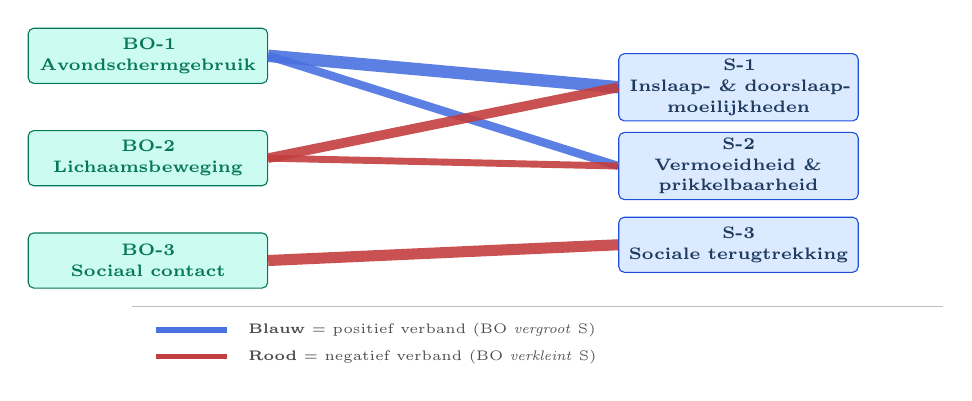
\begin{tikzpicture}[node distance=0pt]
  \node[smprnode] (bo1) at (0, 1.3)  {BO-1\\Avondschermgebruik};
  \node[smprnode] (bo2) at (0, 0.0)  {BO-2\\Lichaamsbeweging};
  \node[smprnode] (bo3) at (0,-1.3)  {BO-3\\Sociaal contact};
  \node[smcrnode] (s1) at (7.5, 0.9) {S-1\\Inslaap- \& doorslaapmoeilijkheden};
  \node[smcrnode] (s2) at (7.5,-0.1) {S-2\\Vermoeidheid \& prikkelbaarheid};
  \node[smcrnode] (s3) at (7.5,-1.1) {S-3\\Sociale terugtrekking};
  \draw[line width=4.5pt, draw=PrimaryBlue!80, opacity=0.90] (bo1.east) -- (s1.west);
  \draw[line width=3.0pt, draw=PrimaryBlue!80, opacity=0.90] (bo1.east) -- (s2.west);
  \draw[line width=3.5pt, draw=StrongRed!85, opacity=0.90] (bo2.east) -- (s1.west);
  \draw[line width=2.5pt, draw=StrongRed!85, opacity=0.90] (bo2.east) -- (s2.west);
  \draw[line width=4.0pt, draw=StrongRed!85, opacity=0.90] (bo3.east) -- (s3.west);
  \draw[line width=0.3pt, draw=black!25] (-0.2,-1.88) -- (10.1,-1.88);
  \draw[line width=2.0pt, draw=PrimaryBlue!80] (0.1,-2.18) -- (1.0,-2.18);
  \node[font=\fontsize{5.5}{7}\selectfont, anchor=west, text=black!70] at (1.15,-2.18) {\textbf{Blauw} = positief verband (BO \emph{vergroot} S)};
  \draw[line width=2.0pt, draw=StrongRed!85] (0.1,-2.52) -- (1.0,-2.52);
  \node[font=\fontsize{5.5}{7}\selectfont, anchor=west, text=black!70] at (1.15,-2.52) {\textbf{Rood} = negatief verband (BO \emph{verkleint} S)};
\end{tikzpicture}
\end{center}

\medskip
\textbf{Prioriteringsredenering (voorbeeld):}
\begin{enumerate}[topsep=2pt,itemsep=1pt,label=\arabic*.]
\item \textbf{BO-1 (Avondschermgebruik)} -- raakt S-1 en S-2 via sterke blauwe verbanden;
monitoring toont 18/21 avonden hoge schermtijd $\rightarrow$ \textbf{prioriteit 1}.
\item \textbf{BO-2 (Lichaamsbeweging)} -- beschermend effect op S-1 en S-2 (rode verbanden);
frequentie extreem laag (0,8/week) $\rightarrow$ \textbf{prioriteit 2}.
\item \textbf{BO-3 (Sociaal contact)} -- sterk negatief verband met S-3; eveneens laag
(0,9/week) $\rightarrow$ \textbf{prioriteit 3}.
\end{enumerate}
\end{voorbeeldbox}

\vspace{0.5em}

\newpage
\subsection*{Casus 1: 25-jarige postgraduaatsstudent -- Deel 3}

\begin{complaintbox}[title={Casus 1: 25-jarige postgraduaatsstudent}]
\small Intrusieve schadeobsessies, compulsieve mentale controle, situationele vermijding en tijdsbelasting door OCD-rituelen. Duur: 18 maanden.
\end{complaintbox}

\begin{monitorbox}
\small\textbf{21-daagse monitoring:} Compulsieve mentale controles en rituelen: gem.\ 3,1 uur/dag (21/21 dagen). Geruststellingszoekend gedrag: gem.\ 4,3 keer/dag. Vermijdingsepisodes (angstgerelateerde situaties niet betreden): gem.\ 2,8/dag. Compulsie-uitstelpogingen: gem.\ 0,4/dag. Gemiddelde slaaptijd: 6,2 uur/nacht.
\end{monitorbox}

\begin{center}
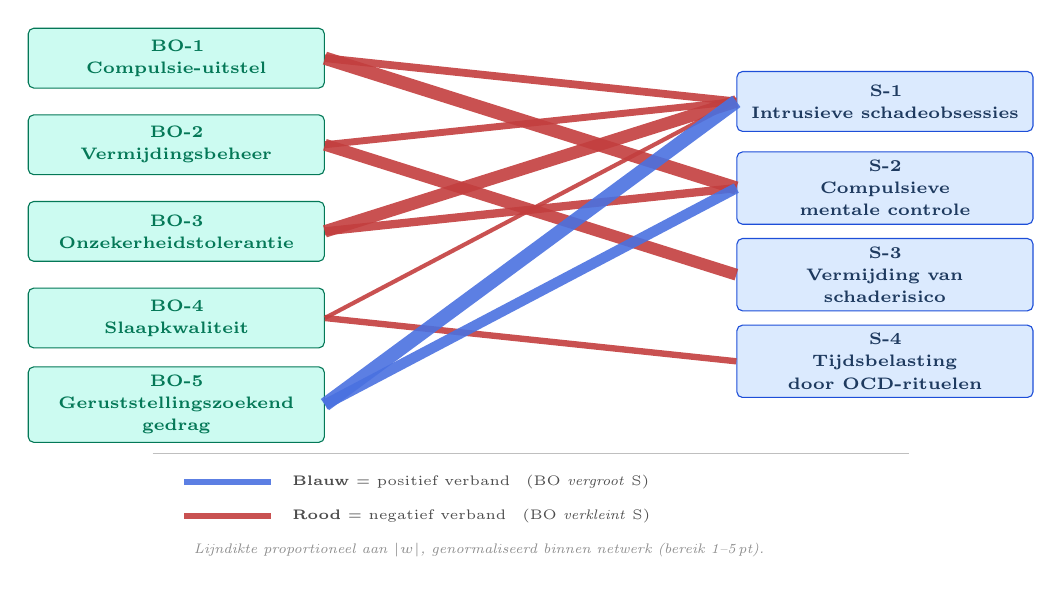
\begin{tikzpicture}[node distance=0pt]
  \node[prnode] (p1) at (0, 2.2) {BO-1\\Compulsie-uitstel};
  \node[prnode] (p2) at (0, 1.1) {BO-2\\Vermijdingsbeheer};
  \node[prnode] (p3) at (0, 0.0) {BO-3\\Onzekerheidstolerantie};
  \node[prnode] (p4) at (0,-1.1) {BO-4\\Slaapkwaliteit};
  \node[prnode] (p5) at (0,-2.2) {BO-5\\Geruststellingszoekend gedrag};
  \node[crnode] (cr1) at (9, 1.65) {S-1\\Intrusieve schadeobsessies};
  \node[crnode] (cr2) at (9, 0.55) {S-2\\Compulsieve mentale controle};
  \node[crnode] (cr3) at (9,-0.55) {S-3\\Vermijding van schaderisico};
  \node[crnode] (cr4) at (9,-1.65) {S-4\\Tijdsbelasting door OCD-rituelen};
  \draw[line width=4.8pt, draw=StrongRed!85, opacity=0.90] (p1.east) -- (cr2.west);
  \draw[line width=2.8pt, draw=StrongRed!85, opacity=0.90] (p1.east) -- (cr1.west);
  \draw[line width=4.3pt, draw=StrongRed!85, opacity=0.90] (p2.east) -- (cr3.west);
  \draw[line width=2.5pt, draw=StrongRed!85, opacity=0.90] (p2.east) -- (cr1.west);
  \draw[line width=4.5pt, draw=StrongRed!85, opacity=0.90] (p3.east) -- (cr1.west);
  \draw[line width=3.0pt, draw=StrongRed!85, opacity=0.90] (p3.east) -- (cr2.west);
  \draw[line width=2.3pt, draw=StrongRed!85, opacity=0.90] (p4.east) -- (cr4.west);
  \draw[line width=1.5pt, draw=StrongRed!85, opacity=0.90] (p4.east) -- (cr1.west);
  \draw[line width=5.0pt, draw=PrimaryBlue!80, opacity=0.90] (p5.east) -- (cr1.west);
  \draw[line width=3.8pt, draw=PrimaryBlue!80, opacity=0.90] (p5.east) -- (cr2.west);
  \draw[line width=0.3pt, draw=black!25] (-0.3,-2.82) -- (9.3,-2.82);
  \draw[line width=2.2pt, draw=PrimaryBlue!80, opacity=0.90] (0.1,-3.18) -- (1.2,-3.18);
  \node[font=\fontsize{5.5}{7}\selectfont, anchor=west, text=black!70] at (1.35,-3.18) {\textbf{Blauw} = positief verband \enspace (BO \emph{vergroot} S)};
  \draw[line width=2.2pt, draw=StrongRed!85, opacity=0.90] (0.1,-3.62) -- (1.2,-3.62);
  \node[font=\fontsize{5.5}{7}\selectfont, anchor=west, text=black!70] at (1.35,-3.62) {\textbf{Rood} = negatief verband \enspace (BO \emph{verkleint} S)};
  \node[font=\fontsize{5.0}{6.5}\selectfont, anchor=west, text=black!45] at (0.1,-4.05) {\textit{Lijndikte proportioneel aan $|w|$, genormaliseerd binnen netwerk (bereik 1--5\,pt).}};
\end{tikzpicture}
\end{center}

\begin{responsebox}
\small\textbf{Opdracht:} rangschik \textbf{alle 5 behandelingsopties} van hoogste naar laagste behandelprioriteit.

\noindent\textbf{Beschikbare behandelingsopties:}\enspace
\textbf{BO-1: Compulsie-uitstel},\quad
\textbf{BO-2: Vermijdingsbeheer},\quad
\textbf{BO-3: Onzekerheidstolerantie},\quad
\textbf{BO-4: Slaapkwaliteit},\quad
\textbf{BO-5: Geruststellingszoekend gedrag}

\rankbox{1}
\rankbox{2}
\rankbox{3}
\rankbox{4}
\rankbox{5}
\end{responsebox}

\vspace{0.6em}
\newpage


% ══════════════════════════════════════════════════════════════════════════════
\section{Deel 4: Verfijnd observatiemodel -- selectie van sub-behandelingsopties}

\begin{tcolorbox}[colback=purple!4,colframe=RichPurple,arc=2.5mm,boxrule=0.9pt,
  left=10pt,right=10pt,top=9pt,bottom=9pt]
\textbf{\color{RichPurple}Instructies Deel 4}

\smallskip\small
\textbf{Opdracht:} selecteer per casus \textbf{exact 6 EMA-items}:
\textbf{2 sub-behandelingsopties per behandeldoel} (3 behandeldoelen $\times$ 2 = 6 items).

\textbf{Wat zijn sub-behandelingsopties?}
De gestandaardiseerde behandeldoelen in dit deel zijn \emph{abstracte domeinen}
(bijv.\ ``Slaapkwaliteit'' of ``Voedingskwaliteit'').
Om dit domein dagelijks via EMA te monitoren, moet het vertaald worden naar
\emph{concrete, specifieke gedragsitems} -- de \textbf{sub-behandelingsopties}.

\textbf{Hoe werkt de abstracte-naar-concrete vertaling?}
\begin{itemize}[topsep=2pt,itemsep=1pt]
\item Een abstract behandeldoel beschrijft een \emph{gedragsdomein} (bijv.\ Slaapkwaliteit, Voedingskwaliteit).
\item Een sub-behandelingsoptie is de \emph{concrete gedragsoperationalisering} van dat domein: een specifiek, dagelijks meetbaar item dat het domein direct meet (bijv.\ ``schermvrij interval voor slapengaan (min)'' als sub-optie van ``Slaapkwaliteit'', of ``gezonde maaltijd genuttigd (ja/nee)'' als sub-optie van ``Voedingskwaliteit'').
\item Selecteer per behandeldoel de 2 items die het domein het \emph{meest direct en precies} meten.
\item Vermijd items die het domein slechts \emph{zijdelings} raken -- zelfs als ze op het eerste zicht verwant lijken.
\end{itemize}

\textbf{Belangrijk:} alle 20 items in de lijst zijn behandelingsoptie-type EMA-items
(modificeerbare gedragingen en strategieen -- \emph{geen} symptomen).
Uw taak is te selecteren welke 6 items het best aansluiten bij de 3 gestandaardiseerde
behandeldoelen, 2 per doel.

\textbf{Antwoordformat:} vink \textbf{exact 6} items aan. Geen toelichting vereist.

\medskip
\textit{\textbf{Zie het uitgewerkte voorbeeld hieronder} voor een concrete illustratie van de selectielogica.}
\end{tcolorbox}

\vspace{0.5em}
\nopagebreak[4]

% ── VOORBEELD DEEL 4 ─────────────────────────────────────────────────────────
\begin{voorbeeldbox}{Deel 4: Verfijnd observatiemodel}{Hoe selecteert u de meest passende EMA-items per behandeldoel?}
\small
\textbf{Gestandaardiseerde behandeldoelen (abstract, voorbeeld):}
\begin{enumerate}[topsep=2pt,itemsep=1pt,label=\arabic*.]
\item Slaapkwaliteit
\item Lichamelijke activiteit
\item Sociaal contact
\end{enumerate}

\textbf{Selectielogica -- hoe kiest u de 2 beste items per doel?}

Stel: doel 1 = \textit{Slaapkwaliteit}. U ziet de volgende opties in de lijst:
\begin{itemize}[topsep=2pt,itemsep=1pt]
\item \checkmark\ ``Schermvrij interval direct voor slapengaan (min)'' $\rightarrow$ \textbf{juist} (operationaliseert het domein direct)
\item \checkmark\ ``Vaste bedtijd aangehouden (ja/nee)'' $\rightarrow$ \textbf{juist} (complementaire meting: regelmaat)
\item $\times$\ ``Cafeine-inname na 15.00 uur (aantal)'' $\rightarrow$ \textbf{niet juist} (raakt slaap slechts zijdelings, hoort niet bij Slaapkwaliteit)
\item $\times$\ ``Maaltijd op vaste tijden genuttigd (ja/nee)'' $\rightarrow$ \textbf{niet juist} (hoort bij Voedingskwaliteit, niet bij Slaapkwaliteit)
\end{itemize}

\medskip
Correct ingevuld (6 items totaal voor de 3 doelen):
\begin{itemize}[topsep=1pt,itemsep=0pt]
\item Doel 1 $\rightarrow$ ``Schermvrij interval voor slapengaan (min)'' + ``Vaste bedtijd aangehouden (ja/nee)''
\item Doel 2 $\rightarrow$ ``Duur actieve beweging vandaag (min)'' + ``Beweegactiviteit uitgevoerd (ja/nee)''
\item Doel 3 $\rightarrow$ ``Bewust sociaal contact gezocht vandaag (ja/nee)'' + ``Sociale activiteit bijgewoond of gepland (ja/nee)''
\end{itemize}
\end{voorbeeldbox}

\vspace{0.5em}

\newpage
\subsection*{Casus 1: 25-jarige postgraduaatsstudent -- Deel 4}

\begin{contextbox}
\small\textbf{Gestandaardiseerde behandeldoelen (abstract) voor Deel 4:}
\begin{enumerate}[topsep=2pt,itemsep=1pt,label=\arabic*.]
\item \textbf{Compulsie- en ritueeluitstel}\quad\textit{\small (domein: bewust en gradueel uitstellen van mentale controles en rituelen bij obsessionele impuls; vrijwel afwezig in monitoring (0,4/dag))}
\item \textbf{Gedragsexperiment en situatiebetreding}\quad\textit{\small (domein: bewust opzoeken van eerder vermeden situaties als gedragsexperiment; vermijding hoog (2,8/dag))}
\item \textbf{Onzekerheids- en intrusietolerantie}\quad\textit{\small (domein: bewust verdragen van onzekerheid en intrusieve gedachten zonder compulsieve respons; geruststellingsgedrag hoog (4,3/dag))}
\end{enumerate}
\end{contextbox}

\begin{responsebox}
\small\textbf{Opdracht:} selecteer \textbf{exact 6} EMA-items (2 per behandeldoel) die het best aansluiten als sub-behandelingsopties.
\textit{Alle 20 items zijn dagelijkse mobiele EMA-items (behandelingsoptie-type, geen symptomen).}
\textit{In het Word-document kunt u de vakjes ($\square$) omcirkelen of markeren in plaats van aanvinken.}

\checkitemBFS{1}{Slaaptijd gisteravond bijgehouden (uren)}
\checkitemBFS{2}{Compulsieve handeling of mentaal ritueel bewust uitgesteld bij impulsdrang (ja/nee)}
\checkitemBFS{3}{Geruststellingsvraag aan anderen gesteld vandaag (aantal)}
\checkitemBFS{4}{Tijdsduur mentaal ritueel met opzet vertraagd of afgebroken (min)}
\checkitemBFS{5}{Cafeine-inname vandaag (aantal dranken)}
\checkitemBFS{6}{Bewuste ontspanningsoefening of ademhaling uitgevoerd (min)}
\checkitemBFS{7}{Situatie die OCD-angst uitlokt bewust opgezocht of niet verlaten (ja/nee)}
\checkitemBFS{8}{Alcoholinname gisteravond (eenheden)}
\checkitemBFS{9}{Wandeling of lichaamsbeweging vandaag (min)}
\checkitemBFS{10}{Gedragsexperiment volledig doorlopen zonder tussentijdse mentale controle (ja/nee)}
\checkitemBFS{11}{Werkuren vandaag (uren)}
\checkitemBFS{12}{Maaltijd op vaste tijden genuttigd (ja/nee)}
\checkitemBFS{13}{Intrusieve gedachte bewust getolereerd zonder compulsieve of vermijdende reactie (ja/nee)}
\checkitemBFS{14}{Stappentelling overdag (stappen)}
\checkitemBFS{15}{Sociaal contact op eigen initiatief gezocht vandaag (ja/nee)}
\checkitemBFS{16}{Onzekerheid bij OCD-situatie bewust verdragen zonder geruststelling of controle (min)}
\checkitemBFS{17}{Waterinname vandaag (glazen)}
\checkitemBFS{18}{Bewuste mindfulness- of aandachtsoefening uitgevoerd (min)}
\checkitemBFS{19}{Werk-privelimiet bewust aangehouden vandaag (ja/nee)}
\checkitemBFS{20}{Schermtijd voor slapengaan (min)}
\vspace{0.4em}
\noindent\textbf{Totaal geselecteerd:}\hspace{0.5em}\rule{1.2cm}{0.25pt}\hspace{0.2em}/ 6
\end{responsebox}

\vspace{0.6em}
\newpage


% ══════════════════════════════════════════════════════════════════════════════
\section{Deel 5: Gepersonaliseerde mobiele coachingsboodschap (HAPA-kader)}

\begin{tcolorbox}[colback=red!3,colframe=ForestGreen,arc=2.5mm,boxrule=0.9pt,
  left=10pt,right=10pt,top=9pt,bottom=9pt]
\textbf{\color{ForestGreen}Instructies Deel 5}

\smallskip\small
\textbf{Opdracht:} schrijf een korte, rechtstreeks tot de persoon gerichte
coachingsboodschap die in de mobiele applicatie verschijnt.

\textbf{Theoretisch kader -- HAPA:}
PHOENIX gebruikt het \textbf{Health Action Process Approach (HAPA; Schwarzer, 1992)}
om de boodschap af te stemmen op de motivationele fase van de persoon:
\begin{itemize}[topsep=2pt,itemsep=1pt]
\item \textbf{Pre-intentionele fase:} de persoon is nog niet gemotiveerd om te veranderen
$\rightarrow$ focus op risicobewustzijn en uitkomstverwachting.
\item \textbf{Intentionele fase:} de persoon wil veranderen maar heeft nog geen concreet plan
$\rightarrow$ focus op doelstelling en actieplanning.
\item \textbf{Actie-/onderhoudsfase:} de persoon probeert al te veranderen
$\rightarrow$ focus op copingplanning en zelfeffectiviteitsondersteuning.
\end{itemize}
U hoeft de fase niet expliciet te benoemen; gebruik het kader om de toon en inhoud
van uw boodschap te sturen.

\textbf{De boodschap voldoet aan:}
\begin{itemize}[topsep=2pt,itemsep=2pt]
\item \textbf{Lengte:} 2--4 zinnen, compact genoeg voor een mobiel scherm.
\item \textbf{Toon:} warm, direct, professioneel -- geen klinisch jargon of diagnostische labels.
\item \textbf{Inhoud:} adresseert het primaire behandeldoel en de voornaamste barriere;
bevat een concrete, eerstvolgende actie.
\item \textbf{Perspectief:} tweede persoon (``jij'' of formeel ``u'').
\end{itemize}

\medskip
\textit{\textbf{Zie het uitgewerkte voorbeeld hieronder} voor een volledige illustratie.}
\end{tcolorbox}

\vspace{0.5em}
\nopagebreak[4]

% ── VOORBEELD DEEL 5 ─────────────────────────────────────────────────────────
\begin{voorbeeldbox}{Deel 5: Mobiele coachingsboodschap}{Hoe formuleert u een effectieve coachingsboodschap?}
\small
\textbf{Context (voorbeeld):}
\begin{itemize}[topsep=2pt,itemsep=1pt]
\item Primair behandeldoel: avondschermgebruik verminderen
\item Voornaamste barriere: gewoontekracht -- schermgebruik is de enige manier om na het werk te ontspannen (lage zelfeffectiviteit)
\item HAPA-fase: intentioneel (wil veranderen, maar heeft nog geen concreet plan)
\end{itemize}

\medskip
\textbf{Voorbeeldboodschap:}\\[0.2em]
\textit{``Je weet dat je avondscherm je slaap in de weg staat, maar het voelt nog als de makkelijkste manier om te ontspannen na een drukke dag. Leg vanavond je telefoon om 21.30 uur in een andere kamer en vul die laatste twintig minuten met iets anders -- een boek, muziek, of gewoon even niets. Een avond is genoeg om te merken dat het kan.''}

\medskip\small
\textbf{Waarom werkt deze boodschap?}
De boodschap erkent de barriere (gewoontekracht), geeft een concrete actie met tijdstip (21.30u), verlaagt de drempel (``gewoon even niets'') en vergroot de zelfeffectiviteit (``een avond is genoeg'').
\end{voorbeeldbox}

\vspace{0.5em}

\newpage
\subsection*{Casus 1: 25-jarige postgraduaatsstudent -- Deel 5}

\begin{contextbox}
\small\renewcommand{\arraystretch}{1.24}
\begin{tabular}[t]{@{}>{\raggedright\bfseries\color{ForestGreen}\arraybackslash}p{0.27\linewidth}>{\raggedright\arraybackslash}p{0.67\linewidth}@{}}
Primair probleem & OCD met schadeobsessies en compulsieve mentale controle die dagelijks twee tot vier uur opslorpt en het dagelijks functioneren ernstig beperkt. \\[0.15em]
Behandeldoel & Compulsie-uitstel: bewust en gradueel uitstellen van mentale controles en rituelen bij elke obsessionele impulsdrang. \\[0.15em]
Voornaamste barriere & Hoge morele verantwoordelijkheidsbeleving; het nalaten van het ritueel voelt als onverantwoordelijk handelen en roept intense schuld op. \\[0.15em]
Copingstrategie & Implementatie-intentie met vastgelegd uitstelprotocol (bijv.\ 15 minuten wachten), gecombineerd met herattributie van de verantwoordelijkheidsgedachte. \\
\end{tabular}
\end{contextbox}

\begin{responsebox}
\small\textbf{Opdracht:} schrijf hieronder de mobiele coachingsboodschap voor deze casus.
\textit{Formuleer alsof de tekst morgen rechtstreeks op de smartphone van de persoon verschijnt.}

\messagelines
\end{responsebox}

\vspace{0.6em}
\newpage


% ══════════════════════════════════════════════════════════════════════════════
\section{Afronding en terugbezorging}

Dank u voor het invullen van alle vijf delen voor uw toegewezen casus.

\begin{instrbox}[title=Checklist voor terugbezorging]
\begin{itemize}
\item[$\square$] Ik heb in Deel 1 symptoomlabels ingevuld.
\item[$\square$] Ik heb in Deel 2 behandelingsoptielabels ingevuld.
\item[$\square$] Ik heb in Deel 3 alle 5 behandelingsopties gerangschikt.
\item[$\square$] Ik heb in Deel 4 exact 6 EMA-items geselecteerd.
\item[$\square$] Ik heb in Deel 5 een mobiele coachingsboodschap geschreven.
\item[$\square$] Mijn antwoorden weerspiegelen mijn eigen klinische oordeel zonder gebruik van generatieve AI of andere externe hulp.
\item[$\square$] Ik begrijp dat mijn antwoorden geanonimiseerd worden voor analyse.
\end{itemize}
\end{instrbox}

\medskip
Bezorg het ingevulde document terug via e-mail aan:
\begin{center}
\texttt{stijn.vanseveren@ugent.be}\quad met onderwerp:\quad \texttt{PHOENIX-PRE-HCP-PRE-05}
\end{center}

\vspace{0.5em}
\begin{tcolorbox}[colback=AccentBlue,colframe=PrimaryBlue,arc=2mm,boxrule=0.6pt,left=8pt,right=8pt,top=7pt,bottom=7pt]
\small\centering
Na ontvangst worden uw antwoorden geanonimiseerd en opgenomen in het expertreferentiecorpus
voor de latere blind evaluatie van PHOENIX. Hartelijk dank voor uw bijdrage aan dit onderzoek.
\end{tcolorbox}

\end{document}
